% !TeX root = ../../main.tex
% Add the above to each chapter to make compiling the PDF easier in some editors.

\section{IOG}\label{ord:ch3:sec4}

The paper "Interactive Object segmentation with Inside-Outside-Guidance"\cite{Zha20-IOG} published by \citeauthor{Zha20-IOG} \etal in 2020 provides a state-of-the-art method to perform interactive object segmentation.

\subsection{Method Description}\label{ord:ch3:sec1:subsec1}
The execution of this method outputs a binary segmentation for a single object of interest within an image. 
To segment multiple objects in one image, the method has t be applied for each of them sequentially.

\gls{iog} is an interactive segmentation method and hence requires user input. 
The input is given by a three mouse clicks on the object's foreground and on its background.
The procedure is shown in Figure \ref{fig:ch3:sec1:iog} and described in the following:
first, in order to form an \emph{"almost-tight bounding box"}\cite[p. 12235]{Zha20-IOG} two exterior clicks are set at the two diagonal locations corners of the object (top-left and bottom-right or bottom-left and top-right).
Based on these two points the other two corner points are derived, which leads to four points on the background. 
Second, to define the object inside the bounding box a single click around the center of the desired object is made, this click is processed as foreground point. 
The background points \emph{"provide "outside" guidance (indicating the background regions) while the interior click gives an "inside" guidance (indicating the foreground region), thus giving the name \textit{Inside-Outside-Guidance}"}\cite[p. 12235]{Zha20-IOG}.
%TODO how to cite a text with quotes properly?

These three points are preprocessed before they are input to the actual model. To include context from the surrounding region the bounding box is enlarged by $p_{{box}}$ pixels. 
%TODO use parameter later to describe my experimental setup.
In order to focus on the object of interest the enlarged bounding box is cropped and resized to the size of $512 \times 512$ \Unit{px}. 
For background and foreground points, a separate heatmap is created by centering a 2D Gaussian at each point with
%TODO write the Gauss-formula 
% ResGauss := exp(-4 * log(2) * ((Rows-PointRow)*(Rows-PointRow) + (Cols-PointCol)*(Cols-PointCol)) / (GaussSigma * GaussSigma))
\begin{equation} \label{equ:gauss}
	\centering
	Gauss = \frac{\exp{-4 * \log 2 }}{\sigma^{2}}
\end{equation}
The two heatmaps have the size of $512 \times 512$ \Unit{px} and are concatenated with the input RGB image to create a 5-channel input for the model. 

\begin{figure}
	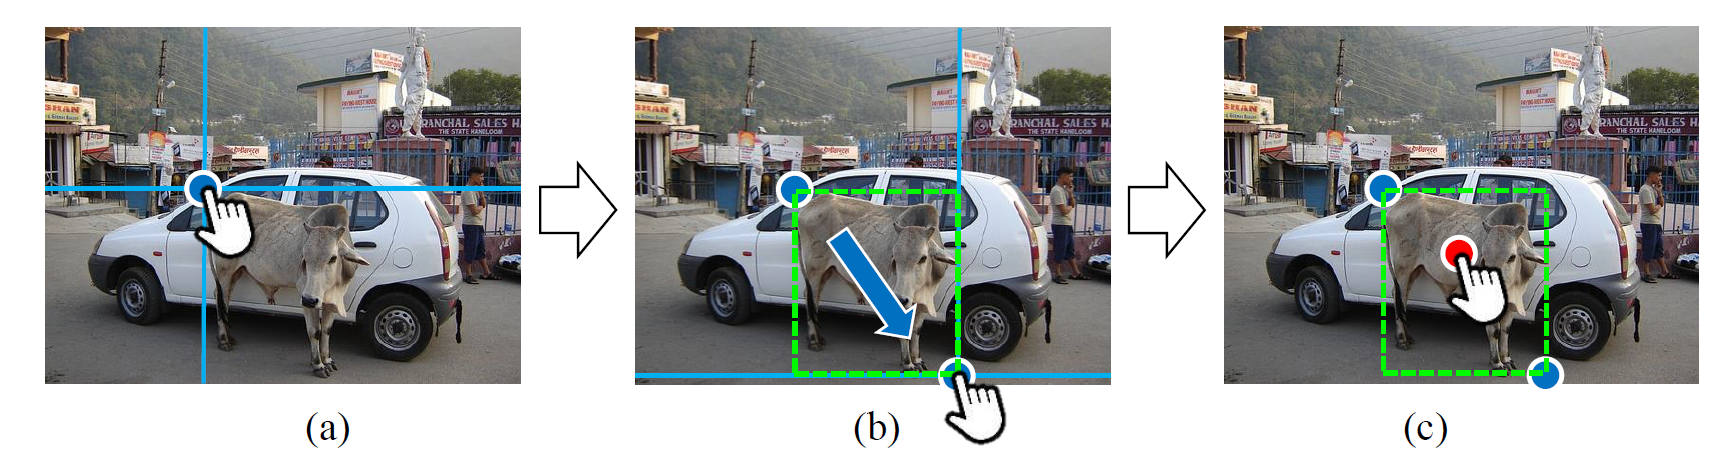
\includegraphics[width=\linewidth]{figures/chap31_clicks.png}
	\caption[IOG Application]{Procedure of setting the three \gls{iog} clicks \cite{Zha20-IOG}. Set the two background clicks (blue) at the diagonal corner locations of the object. Gather a bounding box based on the background clicks. Set a foreground point (red) at the middle of the object.}
	%TODO Bitte die Bildunterschriften so aussagekräftig wie möglich. Ich beginne immer mit einer kurzen Überschrift und beschreibe dann in 2-5 Sätzen was genau gezeigt wird oder was man in der Figure sehen kann. Der Leser tendiert dazu sich zu allererst oder auch nur die Figures anzusehen, daher ist es gut wenn diese für sich stehen und alles wichtige in deren Unterschrift beschrieben wird. Natürlich knapp aber präzise..
	\label{fig:ch3:sec1:iog}
	% TODO Bitte die Bildunterschriften so aussagekräftig wie möglich. Ich beginne immer mit einer kurzen Überschrift und beschreibe dann in 2-5 Sätzen was genau gezeigt wird oder was man in der Figure sehen kann. Der Leser tendiert dazu sich zu allererst oder auch nur die Figures anzusehen, daher ist es gut wenn diese für sich stehen und alles wichtige in deren Unterschrift beschrieben wird. Natürlich knapp aber präzise.
\end{figure}

\subsection{Architecture}\label{ord:ch3:sec1:subsec2}

The architecture of the \gls{iog} method is based on a \emph{"coarse-to-fine design"}\cite[p. 12237]{Zha20-IOG} (see Figure \ref{fig:ch3:sec1:arch}), containing two main parts: the CoarseNet and the FineNet.
%TODO also cite other papers e.g. FPN (feature pyramid networks) or U-Net

\paragraph{CoarseNet}
The CoarseNet contains the heavy encoder part, that mainly consists of a classifier often referred to as backbone. In \gls{iog} a ResNet-101 \cite{He16-ResNet} is used .
% TODO describe backbone and PSP as encoder 
This ResNet-101 is implemented without the head of fully connected layers. It contains four ResNet blocks and the fourth block outputs 2048 feature maps of the size $32 \times 32$ \Unit{px}.
After the backbone a PSP-network is applied in order to enrich "the representation with global contextual information"\cite{Zha20-IOG}.
The coarse prediction from the PSP-Network \cite{Zhao17-PSP} has a spatial dimension of  $32 \times 32$ \Unit{px} with 512 feature maps. 
From this onward the layers are enlarged by a four staged upsampling process to obtain the original input size of  $512 \times 512$ \Unit{px}. 
During the upsampling process activations from the residual parts of the ResNet are transferred from the ResNet using so lateral connections and concatenated with the upsampled feature maps.
%TODO describe this with encoder-decoder 
A benefit of this architecture is the fusion of information from different network stages.

\paragraph{FineNet}
The FineNet is based on a "multi-scale fusion structure"\cite{Zha20-IOG}. 
The activations from all four stages of the upsampling process from the CoarseNet are further processed along different paths. 
Depending on the spatial dimension, a number of additional convolution and upsampling operations are applied in order to use \emph{"features at deeper layers for better trade-off between accuracy and efficiency"} \cite[p. 12237]{Zha20-IOG}.
These different paths are concatenated to create the networks final layer.
A sigmoid is applied to this final layer, which results in a probability map as final prediction of the \gls{iog} network.
The author shows in an ablation study, that the FineNet enhances the networks IoU by $0.8\%$. 
The ablation study is performed with a ResNet-50 as backbone and PASCAL-1k \cite{Eve20-PascalVOC} as dataset. 
\\
This architecture especially performs well due to its application of lateral connections from different levels in order to recover local detail.
The combination of layers with high localization detail with the layers, that contain high detection details, is helpful to prevent a information loss during the down- and upsampling process.

\begin{figure}
	%TODO adapt figure.
	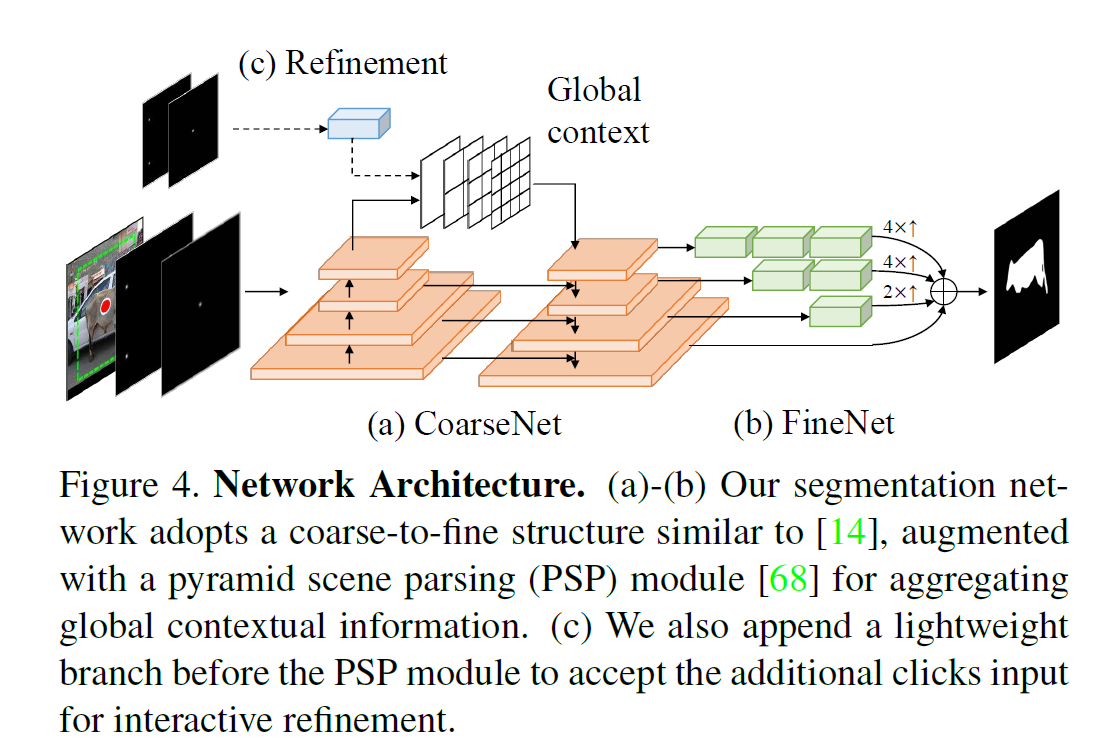
\includegraphics[width=\linewidth]{figures/chap31_arch.png}
	\caption[IOG Architecture]{\gls{iog} architecture (not final).}
	\label{fig:ch3:sec1:arch}
\end{figure}

\subsection{Refinement}\label{ord:ch3:sec1:subsec3}
If a segmentation results does not meet the user's expectations a refinement can be performed iteratively. 
This is done by an additional user click, which can be a fore- or background click on the region with the greatest error. 
In the refinement iteration of the model, this new point is processed in the same way as the initial user click positions to create a heatmap for fore- and background.
These two heatmaps are combined into a two-channel input, which is processed in a so called "lightweight-branch". 
In this branch five convolution operations are applied and the result is concatenated with the ResNet's output of the first iteration.
Hence, the ResNet does not require another execution and leads to a fast refinement process.
Further, the normal \gls{iog} process is executed from the PSP-module. 
Zhang states that the usage of the lightweight-branch performs better than adding the refinement click into the normal 5-channel input.

In their experiments Zhang compares the \gls{iog} method to other state-of-the-art methods on different benchmarks, as shown in Figure %TODO.
They also evaluate the generalization abilities of \gls{iog} on unseen classes.
Zhang claims that \gls{iog} outperforms all other methods.

